%%
%% Class homework & solution template for latex
%% Alex Ihler
%%
\documentclass[twoside,11pt]{article}
\usepackage{amsmath,amsfonts,amssymb,amsthm}
\usepackage{graphicx,color}
\usepackage{verbatim,url}
\usepackage{listings}
\usepackage{upquote}
\usepackage[T1]{fontenc}
%\usepackage{lmodern}
\usepackage[scaled]{beramono}
%\usepackage{textcomp}

% Directories for other source files and images
\newcommand{\bibtexdir}{../bib}
\newcommand{\figdir}{fig}

\newcommand{\E}{\mathrm{E}}
\newcommand{\Var}{\mathrm{Var}}
\newcommand{\N}{\mathcal{N}}
\newcommand{\matlab}{{\sc Matlab}\ }

\setlength{\textheight}{9in} \setlength{\textwidth}{6.5in}
\setlength{\oddsidemargin}{-.25in}  % Centers text.
\setlength{\evensidemargin}{-.25in} %
\setlength{\topmargin}{0in} %
\setlength{\headheight}{0in} %
\setlength{\headsep}{0in} %

\renewcommand{\labelenumi}{(\alph{enumi})}
\renewcommand{\labelenumii}{(\arabic{enumii})}

\theoremstyle{definition}
\newtheorem{MatEx}{M{\scriptsize{ATLAB}} Usage Example}

\definecolor{comments}{rgb}{0,.5,0}
\definecolor{backgnd}{rgb}{.95,.95,.95}
\definecolor{string}{rgb}{.2,.2,.2}
\lstset{language=Matlab}
\lstset{basicstyle=\small\ttfamily,
        mathescape=true,
        emptylines=1, showlines=true,
        backgroundcolor=\color{backgnd},
        commentstyle=\color{comments}\ttfamily, %\rmfamily,
        stringstyle=\color{string}\ttfamily,
        keywordstyle=\ttfamily, %\normalfont,
        showstringspaces=false}
\newcommand{\matp}{\mathbf{\gg}}




\begin{document}

\centerline{\Large Homework 1}
\centerline{Zachary DeStefano, 15247592}
\centerline{CS 274B: Spring \& 2016}
\centerline{\bf Due: April 15, 2016}

\section*{Problem 1: }

I will assume that each random variable can take on $d$ values.

\subsection*{Part A}

To satisfy $p(W|X,Y,Z)$, we need $d-1$ parameters for values of $W$ and each of those values are conditioned on $d^3$ possible configurations of $X,Y,Z$, thus we need $d^3(d-1)$ parameters.\\
\\
To satisfy $p(Z|X,Y)$, we need $d^2(d-1)$ parameters because we have $d-1$ parameter values each conditioned on $d^2$ configurations. \\
\\
To satisfy $p(Y|X)$, we need $d(d-1)$ parameters because we have $d-1$ parameter values each conditioned on $d$ configurations.\\
\\
To satisfy $p(X)$, we need $d-1$ parameters because we have $d-1$ parameter values.\\
\\
Our total is thus
\[
\frac{d^4-1}{d-1}(d-1)
\]
Simplifying, our final total is
\[
d^4-1
\]
Thus this Bayesian network does not simplify the joint distribution
\begin{figure}[h]
\centering
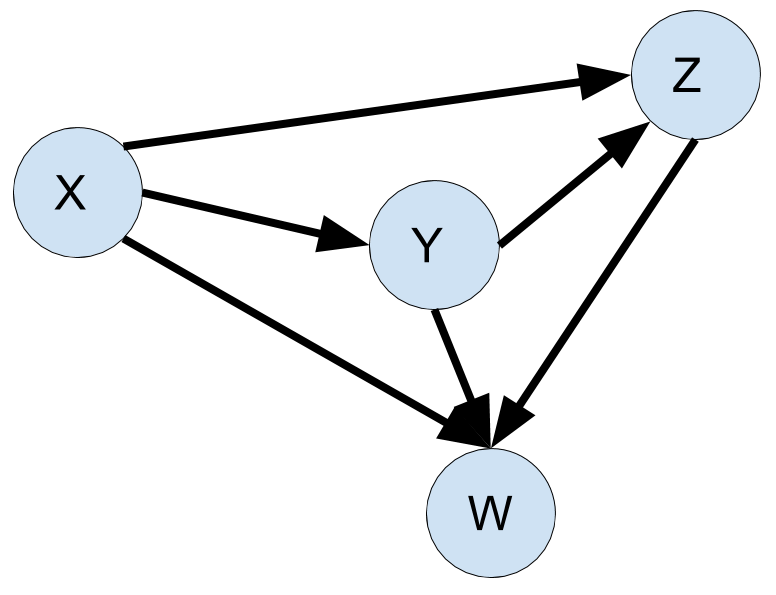
\includegraphics[width=3in]{HW1_Prob1_partA.png}
\caption{Minimal Directed Graphical Model for Part A}
\end{figure}
\newpage
\subsection*{Part B}

For each random variable, we need $d-1$ parameters. \\
They are all independent\\
Thus our total is just $4(d-1)$
\begin{figure}[h]
\centering
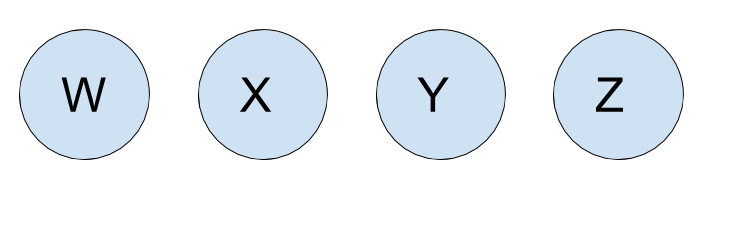
\includegraphics[width=3in]{HW1_Prob1_partB.png}
\caption{Minimal Directed Graphical Model for Part B}
\end{figure}

\subsection*{Part C}

The variables $p(Z|Y)$, $p(W|Y)$, $p(X|Y)$ each need $d(d-1)$ parameters since we have $d-1$ parameter values conditioned on $d$ configurations.\\
\\
The factor $p(Y)$ needs $d-1$ parameters\\
\\
Thus our total is $(3d+1)(d-1)$
\begin{figure}[h]
\centering
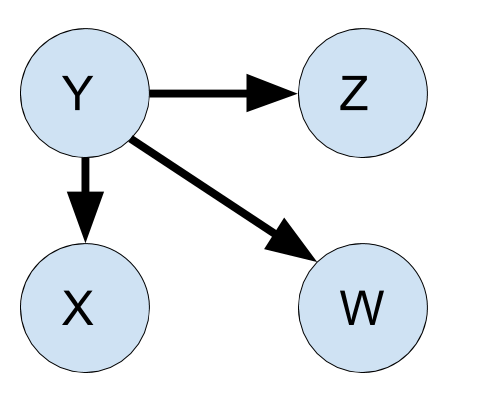
\includegraphics[width=3in]{HW1_Prob1_partC.png}
\caption{Minimal Directed Graphical Model for Part C}
\end{figure}

\newpage

\subsection*{Part D}

To satisfy $p(X)$ and $p(Y)$ we need $d-1$ parameters for each of them\\
\\
To satisfy $p(W|X)$ we need $d(d-1)$ parameters since there are $d-1$ parameter values conditioned on $d$ configurations. \\
To satisfy $p(Z|X,Y)$ we need $d^2(d-1)$ parameters since there are $d-1$ parameter values conditioned on $d^2$ configurations.\\
\\
Our total is thus
\[
(d^2+d+2)(d-1) = (d^2+d+1)(d-1) + (d-1) = (d^3-1) + (d-1) = d^3 + d - 2
\]
\begin{figure}[h]
\centering
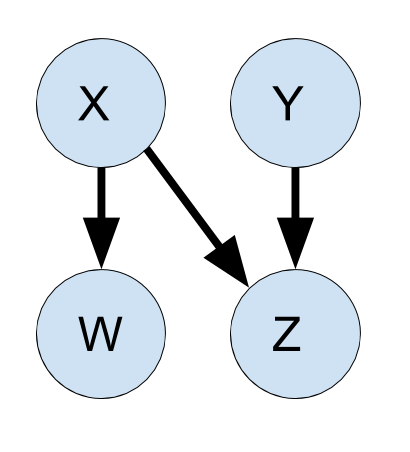
\includegraphics[width=3in]{HW1_Prob1_partD.png}
\caption{Minimal Directed Graphical Model for Part D}
\end{figure}

\newpage

\subsection*{Part E}

To satisfy $p(Z)$ we need $d-1$ parameters\\
\\
To satisfy $p(Y|Z)$ we need $d(d-1)$ parameters as there are $d-1$ values conditioned on $d$ configurations. \\
To satisfy $p(X|Y)$ we need $d(d-1)$ parameters for same reason as $p(Y|Z)$\\
\\
To satisfy $p(W|X)$ we need $d(d-1)$ parameters for same reason as $p(Y|Z)$\\
\\
Our total is thus $(3d+1)(d-1)$ parameters

\begin{figure}[h]
\centering
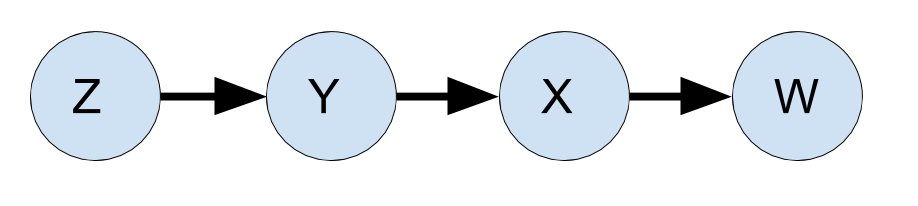
\includegraphics[width=3in]{HW1_Prob1_partE.png}
\caption{Minimal Directed Graphical Model for Part E}
\end{figure}

\subsection*{Part F}

To satisfy $p(X)$ we need $d-1$ parameters\\
To satisfy the other three factors, we need $d(d-1)$ parameters for each of them for the same reason as $p(Y|Z)$ in part E\\
Our total is thus $(3d+1)(d-1)$ parameters

\begin{figure}[h]
\centering
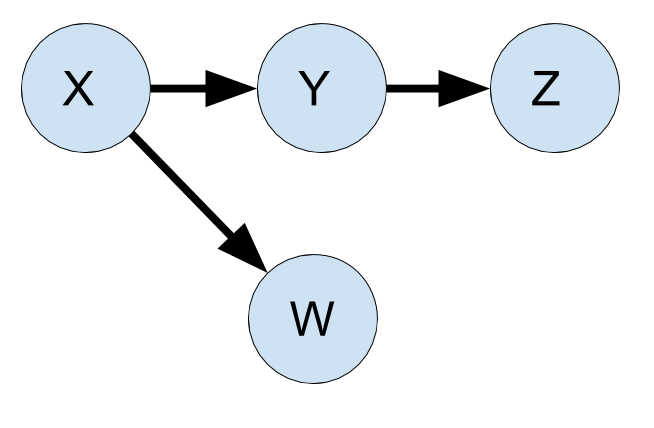
\includegraphics[width=3in]{HW1_Prob1_partF.png}
\caption{Minimal Directed Graphical Model for Part F}
\end{figure}

\newpage

\section*{Problem 2:}

\subsection*{Part A}
Yes\\
Knowing $\textit{projector\_plugged\_in}$ lets you update probabilities for $\textit{power\_in\_wire}$.\\
This in turns means you can infer new probabilities for $\textit{power\_in\_building}$\\
These new probabilities mean you now have new values for  $\textit{room\_light\_on}$\\
This will in turn mean new probabilities for $\textit{Sam\_reading\_book}$

\subsection*{Part B}

Yes\\
This allows you to infer new values for $\textit{power\_in\_building}$\\
This will in turn mean new probabilities for $\textit{Sam\_reading\_book}$\\

\subsection*{Part C}

Yes\\
**ADD EXPLANATION**

\subsection*{Part D}

If $\textit{lamp\_works}$ was observed, then we would update the probabilities for $\textit{projector\_lamp\_on}$\\
We would then have to update the probabilities for $\textit{screen\_lit\_up}$\\
This would cause us to update probabilities for $\textit{ray\_says\_screen\_is\_dark}$\\
**VERIFY THIS**

\subsection*{Part E}

If we observe just $\textit{power\_in\_projector}$ then the same variables from Part D will have their probabilities changed.\\
We would also have to update $\textit{power\_in\_building}$ and $\textit{power\_in\_wire}$\\
**VERIFY THIS**

\newpage

\section*{Problem 3: }

\subsection*{Part A}

We need to solve the following
\[
p(0,0;\theta) + p(0,1;\theta) + p(1,0;\theta) + p(1,1;\theta) = 1
\]
This ends up being the following:
\[
exp(-A(\theta)) + exp(-A(\theta)) + exp(\theta_x - A(\theta)) + exp(\theta_x + \theta_{xy} - A(\theta)) = 1
\]
After doing some factoring
\[
\frac{exp(\theta_x) + exp(\theta_{xy} + \theta_x) + 2}{exp(A(\theta))} = 1
\]
After cross multiplying and solving for $A(\theta)$
\[
A(\theta) = log( exp(\theta_x) + exp(\theta_{xy} + \theta_x) + 2 )
\]

\subsection*{Part B}
After letting $\theta_{xy} = 1$ we have the following
\[
A(\theta) = log( exp(\theta_x) + exp(1 + \theta_x) + 2 )
\]
After some factoring
\[
A(\theta) = log( exp(\theta_x)(1 + exp(1) ) + 2 )
\]
\begin{figure}[h]
\centering
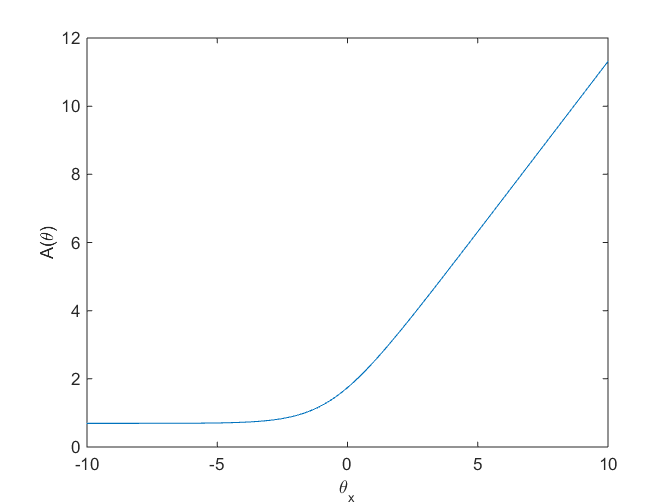
\includegraphics[width=4in]{prob3bplot.png}
\caption{Plot for $A(\theta)$. It appears convex as expected}
\end{figure}

\subsection*{Part C}
This is the partial with respect to $\theta_x$
\[
\frac{\partial A}{\partial \theta_x} = \frac{exp(\theta_x) + exp(\theta_x + \theta_{xy})}{exp(\theta_x) + exp(\theta_x + \theta_{xy}) + 2}
\]
This is the partial with respect to $\theta_{xy}$
\[
\frac{\partial A}{\partial \theta_{xy}} = \frac{exp(\theta_x + \theta_{xy})}{exp(\theta_x) + exp(\theta_x + \theta_{xy}) + 2}
\]
Thus we have 
\[
\bigtriangledown A(\theta) = [\frac{exp(1)+exp(3)}{exp(1)+exp(3)+2},\frac{exp(3)}{exp(1)+exp(3)+2}]
\]
Approximately 
\[
\bigtriangledown A(\theta) = [0.91937,0.80978]
\]
This is also the expected value of the distribution if $\theta=[1,2]$
\end{document}
